\documentclass{article}

\usepackage{graphicx}
% Links
\usepackage[pdftex, colorlinks, urlcolor=blue, linkcolor=black]{hyperref}
% Para el español
\usepackage[spanish]{babel}
\usepackage[utf8]{inputenc}
\spanishplainpercent
% Codigo
\usepackage{listings}
% Para el código en Go.
\usepackage{lstlang0}
% Colores personalizados.
\usepackage{color}
\definecolor{orange}{rgb}{0.99, 0.50, 0.13}
\definecolor{carnelian}{rgb}{0.7, 0.11, 0.11}
\definecolor{cerulean}{rgb}{0.0, 0.48, 0.65}
\definecolor{royalblue}{rgb}{0.0, 0.14, 0.4}
\definecolor{shamrockgreen}{rgb}{0.0, 0.62, 0.38}
% Settings para los fragmentos de código.
\renewcommand{\lstlistingname}{Fragmento}
\lstset{
	language = go,
	tabsize = 4,
	numbers = left,
	%Keywords
	keywordstyle = {[1]\color{orange}\bfseries},
	%Funciones
	keywordstyle = {[2]\color{shamrockgreen}\bfseries},
	%Tipos
	keywordstyle = {[3]\color{royalblue}},
	stringstyle = \color{carnelian},
	commentstyle = \color{cerulean},
	frame = tb,
	showstringspaces = false,
	breaklines = true,
	escapeinside= {\%*}{*)},
	extendedchars= true,
	literate = {ô}{{\^{o}}}1 {ó}{{\'{o}}}1 {á}{{\'{a}}}1 {é}{{\'{e}}}1 {í}{{\'{i}}}1 {ú}{{\'{u}}}1
}

\begin{document}

\begin{figure}
	\centering
	
\includegraphics[width=0.9\linewidth]{./logo_fiuba_alta}
	\label{fig:logo_fiuba_alta}
\end{figure}

\title{Informe sobre GO - Teoría del Lenguaje}
\author{Cristian González \and Tomás Arjovsky}
\date{1$^{er}$ Cuatrimestre, 2015}
\maketitle
\newpage
\tableofcontents
\newpage
\section{Historia}
\subsection{Historia del Proyecto}
El 21 de septiembre de 2007 Robert Griesemer, Rob Pike y Ken Thompson comenzaron a esbozar metas sobre el nuevo lenguaje. A los pocos días los objetivos se habían asentado en proyecto concreto y en idea clara de lo que sería. En enero de 2008 Jen había empezado a trabajar en un compilador para explorar ideas y el cual generaba código en C.
En mayo de 2008, Ian Taylor comenzó de forma independiente en CCG para Go utilizando el borrador de la especificación. Russ Cox se unió a finales de 2008 y ayudó a mover el lenguaje y las bibliotecas del prototipo a realidad.
Go se publica como un proyecto de código abierto el 10 de Noviembre del 2009. 

\subsection{Estado del Proyecto}

Go se convirtió en un proyecto público de código abierto, el 10 de noviembre de 2009. Después de un par de años de diseño y desarrollo, estabilidad Go 1 fue lanzado el 28 de marzo de 2012. Go 1, que incluye una especificación del lenguaje, conjunto de bibliotecas y herramientas personalizadas, proporciona una base estable para la creación de productos fiables, proyectos y publicaciones. 

Con esa estabilidad establecida, Google utiliza Go para desarrollar programas, productos y herramientas en lugar de cambiar activamente el lenguaje y las bibliotecas. De hecho, el objetivo de Go 1 es proporcionar estabilidad a largo plazo. El desarrollo de Go sigue en pie, pero la atención se centra en el rendimiento, fiabilidad, portabilidad y la adición de nuevas funcionalidades como soporte mejorado para la internacionalización.
\subsection{¿Por qué la creación de Go?}

Go nació de la frustración con lenguajes y entornos existentes para la programación de sistemas. La programación había vuelto demasiado difícil y la elección de las lenguas era parte de la culpa. Había que elegir entre la compilación eficiente, eficaz ejecución, o la facilidad de programación; los tres no estaban disponibles en un mismo lenguaje. Los programadores que podría elegían facilidad sobre la seguridad y la eficiencia moviendo a escribirse dinámicamente lenguajes como Python y JavaScript en lugar de C ++ o, en menor medida, de Java. 

Go es un intento de combinar la \textbf{facilidad de programación de un lenguaje interpretado}, \textbf{tipos dinámicos con eficiencia} y \textbf{la seguridad de un lenguaje compilado estáticamente}. 

Por último, se pretende que ser rápido: debe tener como máximo unos segundos para construir un gran ejecutable en un solo equipo. Para cumplir con estos objetivos se requieren abordar una serie de cuestiones lingüísticas: un sistema de tipo expresivo, pero ligero; concurrencia y un buen recolector de basura; especificación de la dependencia rígida; etcétera.

\section{Sintaxis Básica}
\subsection{Paquetes}
Cada archivo de código fuente, independientemente de su nombre, aclara en la primera línea a qué paquete pertenece.

Si se quiere acceder desde un paquete a otro, lo que se hace es importar su path. Por convención, los paquetes se llaman como el último elemento del path. Importar un paquete permite usar los nombres que este exporta, típicamente funciones o variables globales (al paquete). Para señalar que un elemento se exporta, su nombre comienza con mayúscula.

Un proyecto comienza a ejecutarse en la función main del paquete main.

\lstinputlisting[caption="Hello World en Go"]{codigo/helloWorld.go}

Se puede importar más de un paquete con la forma factoreada. Esta forma es utilizada también para otras keywords además de import, como var.

\begin{lstlisting}[caption=Forma Factoreada]
import (
	"fmt" 
	"math"
)
\end{lstlisting}

\subsection{Variables}
Las variables en Go son declaradas de forma inversa al C, pareciéndose más a la de Pascal. Esta decisión fue tomada por los creadores principalmente por la dificultad para entender en C los tipos compuestos con punteros y las funciones de alto orden\cite{dec}.
\begin{description}
	\item[Declaración:]\hfill \\
		\lstinline|var a,b,c int|
	\item[Inicialización en declaración:] \hfill \\
		\lstinline|var a,b,c int = 1,2,3 // Hay asignación múltiple!|
	\item[Inferencia de Tipos:] para constantes y variables. \\
		\lstinline|var c = 1 // c pasa a ser de tipo int.|
	\item[Forma Compacta:] \hfill \\
		\lstinline|c := 1 // c se declara y se asigna.|
	
	Esta forma se puede usar siempre y cuando se esté dentro de una función (main incluida). Esto se debe a que globalmente (a nivel paquete) todas las líneas deben empezar con alguna keyword. 
	\item[Forma Factoreada:] La keyword \lstinline|var| también admite forma factoreada.
\begin{lstlisting}
var (
	a = 3 // inferencia sobre constante.
	b = a // inferencia sobre variable que ya tiene tipo.
)
\end{lstlisting}
\end{description}

Al asignar en Go una variable a la otra, se asigna el valor, al estilo imperativo, con lo cual cambiar una no tendrá ningún efecto sobre la otra (como sí sucedería en los lenguajes como Java, donde las variables son referencias).

Los punteros se declaran de la forma \lstinline|var a *int|. A diferencia de C, \emph{no hay aritmética de punteros}. Esta omisión fue pensada para aumentar la seguridad (evitar direcciones ilegales) y simplificar la implementación del recolector de basura.\cite{pa}
%TODO ver el tema del make, que no se puede hacer personalizado.

\subsection{Funciones}
No se declaran a través de su tipo de retorno, como se hace en C, sino que tienen la keyword \lstinline|func|.
\begin{description}
	\item[Declaración:]\hfill \\
		\lstinline|func nombre(a tA, b tB,...) tRet {...}| 
	\item[Argumentos agrupados según tipo:] \hfill \\
		\lstinline|func nombre(a, b int) int {...}|
	\item[Retorno Múltiple:] compatible con la asignación múltiple. \\
		\lstinline|func swap(a, b int) int {return b,a}|
	\item[Return Values como variables:] se pueden modificar en el interior de la función y al final usar "return" las devuelve en el orden especificado en la firma.
\begin{lstlisting}[caption = una variable elevada al cuadrado 3 veces]
func primeros3Cuadrados.(a int) m1,m2,m3 int{
	m1 = a*a
	m2 = m1*m1
	m3 = m2*m2
	return
}
\end{lstlisting}
\end{description}

\subsection{Estructuras de Control}
\subsubsection{Loops: for}
La única estructura de control de ciclos en Go es el \lstinline|for|, que es lo suficientemente flexible y cómodo como para reemplazar al while(), do{}While() y otros. Una diferencia menor es que los paréntesis ya no se usan y las llaves son obligatorias.
\begin{description}
	\item[Forma clásica:] \hfill \\
		\lstinline|for i := 0; i < 10; i++ { fmt.Println(i) }|
	\item[Omisiones:] El pre y el post pueden no ponerse (cualquier combinación es válida). Cuando queda solo la condición de corte, se da el caso que reemplaza al while: \\
		\lstinline|for a < 1000 { a = a*a }|
	\item[range:] para operar sobre arrays y slices (más adelante se ven), se puede usar \lstinline|range|. Es una forma primitiva que, junto a la función \lstinline|len|, elimina la necesidad de máximos lógicos, constantes o variables referidas al tamaño. Se pueden omitir el índice o el valor con el operador \_:
	\begin{itemize}
	\item \lstinline|for i,v := range arreglo {fmt.Println("indice:",i,"valor:",v)}|
	\item \lstinline|for i := range arreglo {fmt.Println("indice:",i)}|
	\item \lstinline|for _,v := range arreglo {fmt.Println("valor:",v)}|
	\end{itemize}
\end{description}
\subsubsection{if}
Igual que el clásico de C o C++, solo que se sigue el mismo criterio con los paréntesis y las llaves y se puede agregar un pre (paso inicial, previo al if), al igual que en el for. De la misma forma, \emph{cualquier variable definida en el pre vivirá solo en el scope del if (y del else)}. %TODO ver si hay otra forma de decir pre y post.
\begin{lstlisting}[caption = promedio precalculado.]
// Al calcular p en el pre, no hay que calcularlo de nuevo adentro del if.
if p := prom(notas); p >= 7 {
	fmt.Println("Aprobado. Promedio:", p)
} else {
	fmt.Println("Reprobado. Promedio:", p)
}
\end{lstlisting}

\subsubsection{switch}
Se agrega un break automático al final de cada case. Entonces, a diferencia de C, para casos múltiples, en lugar de omitir un break, se hacen conjuntos separados por coma. Además, las expresiones de cada caso son más generales, ya que no necesitan ser constantes o siquiera enteros. 

\begin{lstlisting}[caption = parsear acciones de T.E.G. (switch sobre strings)]
switch accion {
	case "invadir": invadir(objetivo)
	case "reagrupar": reagrupar()
	case "pedir tarjeta", "tarjeta": sacarCarta(mazo)
	default: fmt.Println("Opción desconocida")
}
\end{lstlisting}
Si no se especifica ninguna variable en el switch se asume \lstinline|switch true|, con lo cual se evalúan expresiones booleanas. Como los casos se evalúan de arriba hacia abajo en orden, el switch a secas es una forma prolija de anidar ifs.

\begin{lstlisting}[caption = switch como ifs anidados.]
switch {
	p < 4: fmt.Println("aplazado")
	p < 7: fmt.Println("reprobado")
	default: fmt.Println("aprobado")
}
\end{lstlisting}

\subsubsection{defer}
Una función a la que se le antepone \lstinline|defer| (posponer, diferir) se ejecuta al final de la función que la contiene. Si hay \lstinline|defer| con más de una función, se ejecutan de forma LIFO.

\lstinputlisting[firstline = 5, caption = Hello World Alternativo]{codigo/defer.go}

Una gran utilidad del defer es, dentro de las funciones que tienen muchos return en distintas circunstancias, usar una función diferida que tiene que ejecutarse en todos los casos de devolución, como por ejemplo, cerrar un archivo. \cite{defer}

\section{Tipos de datos}
Go tiene tipado estático (en tiempo de compilación) y fuerte. Las variables o bien son declaradas con un cierto tipo o lo infieren de la parte derecha de una asignación, luego de lo cual no pueden cambiar su tipo. Lo más parecido a tipado dinámico son las interfaces, que se verán más adelante.

Estos son los tipos básicos de Go:
\begin{description}
\item[Booleanos:] \lstinline|bool|.
\item[Cadenas:] \lstinline|string|.
\item[Enteros:] \lstinline|int  int8  int16  int32  int64|.
\item[Sin signo:] \lstinline|uint uint8 uint16 uint32 uint64 uintptr|.
\item[Bytes:] \lstinline|byte|. Alias de uint8.
\item[Caracteres:] \lstinline|rune|. Alias de int32, se verá más adelante, representa un punto de Unicode.
\item[Flotantes:] \lstinline|float32 float64|
\item[Complejos:] \lstinline|complex64 complex128|
\end{description}

Cada tipo tiene un \emph{zero value}, que es un valor en el que se inicializa la variable si no se especifica uno al declararla. Para los valores numéricos es 0, para las strings, la cadena vacía y para estructuras complejas suele ser nil.

%TODO ver casos raros para inferencia, como variables que todavía no tienen valor, y demás.
La \emph{inferencia} es bastante simple, ya que es un lenguaje tipado. Cuando se usa el operador := con una variable del lado derecho, la del lado izquierdo adquiere su mismo tipo. 

El caso más raro es el de las constantes numéricas, que son de alta precisión y no tienen un tipo, sino que proveen el tipo necesario para las operaciones que se hagan sobre ellas. 
\lstinputlisting[caption = Constantes Comodines]{codigo/constantes.go}
El caso anterior produce el siguiente output: 
\begin{verbatim}
La variable es de tipo int y tiene valor: 5.
La variable es de tipo float32 y tiene valor: 5.
La variable es de tipo float32 y tiene valor: 5e+19.
\end{verbatim}
Esto muestra justamente lo propuesto de que la constante provee el tipo necesitado. Sin embargo, esto tiene sus excepciones, como es el caso de c2. Esta constante es un número muy grande como para  proveer un valor de tipo int, con lo cual si se quitan las barras de comentario de la última línea del main, el programa falla en tiempo de compilación: 

\begin{verbatim}
./constantes.go:20: constant 50000000000000000000 overflows int
\end{verbatim}

Como se decía antes, hay que notar que este comportamiento de comodín es \emph{solo para constantes}. La conversión de tipos entre variables es \emph{siempre explícita}.

\lstinputlisting[caption = asignación ilegal.]{codigo/variables.go}
Produce el siguiente mensaje de error:
\begin{verbatim}
./variables.go:6: cannot use entera (type int) as type float32
 in assignment
\end{verbatim}
Para hacerlo correctamente hay que explicitar la conversión:
\lstinputlisting[caption = conversión legal.]{codigo/variablesbien.go}

Si creamos tipos propios o queremos hacer funciones que conviertan de un tipo a otro que son muy distintos, podemos hacer uso de interfaces, reflexión y switches sobre tipos. Más adelante %TODO linkear
se explica este caso.

En adelante se detallan algunos tipos de datos específicos:

\subsection{Structs}
Prácticamente iguales a los de C. Para usarlos, se define un tipo basado en struct de la siguiente manera:
\begin{lstlisting}[caption = declaración de structs]
type vertice struct{
	x int
	y int
	z int
}
\end{lstlisting}

Son la forma empaquetada nativa de Go. Se pueden asignar structs literales de la siguiente forma: \lstinline| v := vertice{1,2,3}|. Se puede inicializar un campo específico (\lstinline|v := vertice{x:1, z:2}|) y los que queden sin asignar tendrán zero values.

Para acceder a sus campos se usa, por ejemplo para el x, v.x.

\paragraph{Transparencia de punteros:} los punteros a registros son transparentes para el acceso a los campos:

\begin{lstlisting}[caption = transparencia de punteros.]
pv := &vertice{10,20,30} // se crea un puntero a un vertice.
fmt.Println(pv.x) // se imprime el primer campo (10).
\end{lstlisting}
\subsection{Arrays}
La forma básica de almacenamiento secuencial. Más allá de su implementación interna, una variable que es un array, \emph{no es un puntero}. Si se hace un puntero al array no apunta a su primer elemento, si no a la variable que lo contiene (recordar que no hay aritmética de punteros).
\begin{description}
	\item[Declaracion:] \hfill \\
	\lstinline|var arr [5]int // 5 es el "element count"|\\
	Es importante tener en cuenta que el element count es parte del tipo: [5]int y [6]int son tipos diferentes.
	\item[Literales:] \hfill \\
		\lstinline|arr := [5]int{1,2,3,4,5}|
	\item[Conteo automático:] a través del operador ``...'' \\
		\lstinline|arr := [...]int{1,2,3,4,5}|
	\item[Inicialización por default:]  si a un array no se le especifican valores con una inicialización, todas sus posiciones son inicializadas en el zero value del tipo base.
	\item[Longitud:] es parte de la variable y se accede a ella con la función \lstinline|len(arr)|
\end{description}

\subsection{Slices}
Forma dinámica secuencial nativa de Go. Se llaman ``slices'' (porciones) porque una de las formas de crearlas es por ``cortando'' un array. Como son dinámicas (pueden crecer en tamaño) tienen dos atributos, longitud (\lstinline|len|) y capacidad (\lstinline|cap|). %TODO bajar redundancia acá.
\begin{description}
	\item[Creación:] al igual que otras estructuras complejas, se crean con la función \lstinline|make|, especificando la longitud (tamaño inicial) y la capacidad (hasta donde pueden crecer sin pedir memoria):
	\begin{itemize}
		\item \lstinline|s := make([]int,5)   // len=5 cap=5|
		\item \lstinline|s := make([]int,0,5) // len=0 cap=5|
	\end{itemize}
	Así como el tipo de los arrays de enteros es [n]int, el de las slices es []int, donde no se especifica el tamaño. Esto significa que una slice de 20 elementos es del mismo tipo que una de 30. El tipo de la variable a crear es siempre el primer argumento de \lstinline|make|.
	\item[Literales:] \hfill \\
		\lstinline|s := []int{1,2,3} // crea una slice de ints con len=3, cap=3|
	\item[Cortando (slicing) arrays:] se especifica el índice del primer elemento (inclusivo) y el último (no inclusivo). Esta diferencia surge de la conveniencia para ver rápidamente el tamaño de la slice restando el segundo número por el primero. O sea, si la slice tiene índices [a,b), entonces su longitud será b - a.
\begin{lstlisting}[caption = slices desde arrays]
a := [...]int{1,2,3,4,5}
s := a[2:4] // s == [3,4]
\end{lstlisting}	
\end{description}

En el caso particular de sacar slices de arrays, los datos no se duplican: los elementos de la slice corresponden a la misma porción de memoria\cite{slices}. Por lo tanto, al modificar una estructura se modifica la otra, y vice-versa. Esto, sin embargo, no hace que sean iguales, o siquiera comparables: las slices solo pueden usar el operador == con un \lstinline|nil| del otro lado. El \lstinline|nil|, justamente, es el zero value de este tipo de datos, y representa una slice vacía.

\paragraph{Re-Slice:} una slice puede ser cortada de nuevo, ya sea en porciones más pequeñas, o más grandes.
\begin{lstlisting}[caption = cortando hacia derecha o hacia izquierda.]
s1 := []int{1,2,3,4}
s2 := s1[:2] // s2 es [1,2] tiene capacidad 4.
s3 := s2[:3] // s3 es [1,2,3] con capacidad 4.
s4 := s1[2:] // s4 es [3,4] tiene capacidad 2.
\end{lstlisting}
En el caso anterior, s2 y s4 son cortes más pequeños que el original, mientras que s3 es un corte más grande (mayor \lstinline|len|) a s2, del cual viene. Una limitación:
\begin{lstlisting}[caption = re-slice ilegal.]
s1 := []int{1,2,3,4}
s2 := s1[:5]
\end{lstlisting}
Si se intentara cortar hacia afuera más allá de la capacidad, esto produce un error en tiempo de ejecución, ya que es un tipo secuencial y más allá de su capacidad puede haber memoria reservada.

\paragraph{Redimensión:} como se ha dicho, la slice es un tipo dinámico, y si se quiere aumentar la capacidad del mismo, esto se hace (internamente) creando una slice nueva con una capacidad mayor y copiando elemento a elemento\cite{slices} con la función \lstinline|copy|. Externamente, sin embargo, existe la función \lstinline|append|, que agrega un elemento al final de la slice, y si sobrepasa la capacidad, se encarga de reubicarla según lo recién descripto.
\begin{lstlisting}[caption = append]
var s1 []int // s1 == nil
s1 = append(s1, 2, 3, 5, 7) // append a un nil es como a una lista vacía.
s2 := []int{10, 20, 30}
s3 := append(s2,s1...) // el operador ... expande s1 para pasar elemento por elemento.
s3[5] = 4
fmt.Println(s1, s3)
\end{lstlisting}
Esto produce como output:
\begin{verbatim}
[2 3 5 7] [10 20 30 2 3 4 7]
\end{verbatim}
Al modificar s3[5] no se modifica s1, ya que lo que se agrega a s3 en el append no es s1 en sí, sino sus elemntos uno a uno con el operador ``...''.

Las funciones \lstinline|copy|, \lstinline|append|, \lstinline|len| y \lstinline|cap| están implementadas de forma abierta, desempaquetada y declarativa, ya que nunca se modifica el original, sino que se devuelve la versión modificada. Sin embargo, el tipo de datos posee estado mutable, lo que se ve sencillamente cambiando el valor de un elemento como en la línea 5 del anterior fragmento de código. Este estilo mixto es muy característico de los tipos de datos estructurados de Go.
\subsection{Runas y strings}
Go acepta en su código fuente cualquier caracter Unicode. En lugar de caracteres al estilo ``char'', Go tiene runes (alias de uint32), que representan Unicode points. Uno caracter de este tipo puede tener ser de hasta 4 bytes, ya que el conjunto incluye símbolos Japoneses, árabes, acentos, cirílicos, y muchos otros.

Por otro lado, contrario a muchos lenguajes, las strings no son cadenas de caracteres, si no que son cadenas de bytes (alias de uint8). Para compatibilizar la conversión ida y vuelta entre bytes individuales y puntos de Unicode, que son de 1 a 4 bytes, se usa el encoding UTF-8, que está incorporado nativamente al procesamiento del código fuente de Go.
\lstinputlisting[firstline = 5, caption = ejemplo de byte vs runa.]{codigo/runas.go}
Da como output:
\begin{verbatim}
el valor es Allô! y su longitud es 6
\end{verbatim}
Esto muestra que si bien la palabra ``Allô!'' tiene 5 caracteres, la longitud de la slice de bytes es de 6, lo cual significa que la runa ô ocupa 2 bytes. 

Para ver un detalle de la comparación, \lstinline|range| itera sobre runas, mientras que para ir byte a byte se trata a la string como un array: 
\lstinputlisting[caption = detalle de byte vs runa.]{codigo/detalleRunas.go}
Output:
\begin{verbatim}
Runas:
0: 'M', que es de tipo int32
1: 'i', que es de tipo int32
2: 'r', que es de tipo int32
3: 'á', que es de tipo int32
5: '!', que es de tipo int32
Bytes:
0: 'M', que es de tipo uint8
1: 'i', que es de tipo uint8
2: 'r', que es de tipo uint8
3: 'Ã', que es de tipo uint8
4: '¡', que es de tipo uint8
5: '!', que es de tipo uint8
\end{verbatim}
En el ejemplo anterior se ve, justamente, que si se mira byte a byte, los caracteres de más de un byte de Unicode, el output de aquellos será incomprensible. Esto es lo que ocurre cuando, por ejemplo, en una página en español no está fijado el encoding UTF-8 para traducir de secuencias de bytes a caracteres Unicode. Este encoding, no casualmente, fue inventado por Rob Pike y Ken Thomson \cite{unicode}, dos de los tres creadores del lenguaje Go.
\subsection{Mapas}
Un mapa es un conjunto de pares de claves y valores. Es como un arreglo, pero su tipo de base no son los numeros enteros, sino que puede ser cualquier tipo de Go, nativo o declarado por el usuario. Es similar a los mapas de C++, de python, etc.
\begin{description}
	\item[Declaración:] con make. \\
		\lstinline|m := make(map[string]string)|
	\item[Asignación:] cambiar el valor para una clave, y de no existir la clave, la crea: \\
		\lstinline|m["palabra"] = "conjunto de letras" // Literalmente, un diccionario.|
	\item[Mapas Literales:] del estilo de los structs.
\begin{lstlisting}[caption = metal]
m := map[rune]int{
	'a':1
	'b':2
	'c':3
}
\end{lstlisting}
	\item[Borrar una clave:] \hfill \\
		\lstinline|delete(mapa, clave)|
	\item[Ver el valor de una clave:] es una asignación doble. Por un lado se obtiene la clave y por el otro un booleano que determina si esa clave efectivamente existe en el mapa. Si no se encontró, como clave devuelve el zero value de su tipo. \\
		\lstinline|valor, ok := m[k] // Si se omite el ok solo se devuelve el valor.|
\end{description}

\subsection{Funciones y clausuras}
En Go las funciones son valores, ya que se tratan como ciudadanos de primera clase (First class citizens).
\begin{lstlisting}[caption = asignación y uso.]
f := func(int a, int b) { return a + b }
fmt.Println(f(3,4)) // 7
\end{lstlisting}
Al ser ciudadanos de primer orden, pueden pasarse como argumentos de otras funciones.
\lstinputlisting[firstline = 5, caption = Map con funciones de alto orden.]{codigo/funcionesPorArgumento.go}
Output: 
\begin{verbatim}
[1 4 9 16 25]
[0 1 1 2 2]
\end{verbatim}

\paragraph{Clausuras:} una función que es creada como valor en un momento dado adquiere acceso global a todas las variables en su entorno. En particular, si este entorno muere, sigue viviendo para la función. A este conjunto función-entorno se lo llama ``clausura''.
\lstinputlisting[firstline = 5, caption = función generadora de clausuras.]{codigo/functionValues.go}
Output:\\
\verb|20 30 35|

La función countFrom es una generadora de funciones de enteros en enteros. Cada una de las generadas tendrá como diferencia entre sí el número con el cual se comienza a contar (asignación sum := n). Cada vez que se invoque a countFrom(n) se creará una nueva función contadora a partir de n. Las clausuras usadas de esta manera emulan estado, y es lo que se usa en Oz para el modelo seguro, empaquetado y declarativo de implementación de TDAs.


\subsection{Tipos de Datos en Go según los criterios de Ole Dahl}
El teórico noruego, en su trabajo Structured programming\cite{ole}, junto con Dijkstra y Hoare, estableció una serie de tipos de datos que debían ser representables en un lenguaje de programación. Según los que vimos en clase, los siguientes tienen su correspondiente representación en Go:
\begin{description}
\item[Producto Cartesiano:] El producto cartesiano entre conjuntos produce un conjunto de tuplas con un elemento de cada conjunto. En Go, esta función la cumplen los \emph{structs}.
\item[Unión Disjunta:] esta es la unión entre conjuntos disjuntos. En C es ``union'', aquí hay un equivalente, que son las \emph{interfaces}, vistas más adelante, que agrupan tipos según los métodos.
\item[Funciones discretas finitas:] los \emph{mapas} establecen relaciones entre dos conjuntos cualesquiera, cumpliendo este requerimiento.
\item[Partes de un conjunto (sets):] si bien no hay un tipo de datos nativo, son muy fácilmente representables \emph{con mapas con valores booleanos}. De hecho, esta es la forma recomendada de implementarlos según los creadores\cite{sets}.
\item[Secuencias:] \emph{slices} como listas. Más adelante se verán otras implementaciones con channels. %TODO revisar.
\end{description}

\section{Métodos}
Los métodos son funciones empaquetadas, para un tipo de datos determinado. Es un pequeño acercamiento al diseño orientado a objetos, solo que se declaran y se usan siempre de forma pública.

\paragraph{Declaración:} se le especifica a una función qué tipo será el que reciba el método antes del nombre de la firma. Solo se pueden definir métodos para tipos creados en el paquete. Si se debe hacer métodos para un tipo nativo, se puede hacer un alias.

\lstinputlisting[caption = uso de métodos]{codigo/metodoNorma.go}
Output: \verb|7.0710678118654755|

Sin embargo, más allá de la forma empaquetada, hay que tener en cuenta que el recibidor del método se comporta de la misma manera en la función que si se hubiera pasado como un argumento\cite{method_int}. 
En go, todo parámetro de una función es pasado por valor, con lo cual si se quiere modificar al argumento original, se deberá pasar un puntero. Lo mismo aplica a los métodos, pero con una comodidad añadida: si un método se define para punteros, al llamarlo para ese tipo, el operador de dirección es agregado automáticamente en la compilación\cite{methods_ef}. 

En el siguiente ejemplo se ve una posible implementación de cómo agregar un elemento a una slice. Si hay que agrandarla, se modificará la variable original, con lo cual es necesario que el método sea para punteros. Sin embargo, en el main, se puede mandar el método a \verb|s| directamente por lo explicado anteriormente. 
\lstinputlisting[caption = modificando una slice.]{codigo/metodoAppend.go}
Output: 
\begin{verbatim}
[1 2 3] tiene longitud 3 y capacidad 3
[1 2 3 20] tiene longitud 4 y capacidad 6
\end{verbatim}

\section{Interfaces}
Las interfaces, como se describieron anteriormente, son tipos que agrupan a otros según los métodos que reciben. Son la única forma de unión disjunta en Go.

A diferencia de las interfaces en Java, no se especifica si un tipo implementa o no una interfaz, sino que se chequea en tiempo de compilación si el tipo del lado derecho de la asignación puede o no recibir los métodos. El objetivo de esta decisión era fomentar la definición de interfaces sin preocuparse por cambiar el código en todos los tipos previamente existentes que la implementen\cite{implements}.

\lstinputlisting[caption = uso de interfaces, firstline = 5]{codigo/interfaces.go}
Error al compilar:
\begin{verbatim}
# command-line-arguments
./interfaces.go:37: cannot use c (type camion) as type reidor in assignment:
	camion does not implement reidor (missing reir method)
\end{verbatim}

Cabe aclarar que se diferencian para las interfaces punteros y valores, ya que los métodos se definen para unos o para los otros. Si un método está definido para punteros y a la interfaz se le asigna un valor, el compilador indicará que la variable no implementa el método requerido.

Además de las interfaces definidas por el usuario, hay muchas predefinidas en el lenguaje, con lo cual se pueden crear tipos nuevos que sean utilizables para funciones nativas de Go.

\subsection{Stringers}
Un stringer es todo tipo de datos que pueda representarse como string:
\begin{lstlisting}[caption = firma de stringers]
type Stringer interface{
	String() string
}
\end{lstlisting}
Esta interfaz está definida en el paquete \verb|fmt| y se utiliza en funciones como \verb|Println| y \verb|Printf| para la impresión de variables.

\subsection{Errores}
En Go no hay excepciones propiamente dichas como tipo de datos. Un error es una interfaz que puede representarse a si mismo como string mediante un método Error(). Esta interfaz también pertenece al paquete \verb|fmt| y es una de las que buscan las funciones de impresión para formatear.

\begin{lstlisting}[caption = firma de errores]
type error interface {
    Error() string
}
\end{lstlisting}

En general, cuando una función puede devolver un error, se lo hace por asignación múltiple como último valor de devolución. Si el valor devuelto no es \lstinline|nil|, entonces se maneja el error como sea necesario, a modo de try-catch.

\lstinputlisting[caption = uso de errores, firstline = 5]{codigo/errores.go}
Output: 
\begin{verbatim}
Fuera de rango: no se puede colocar el elemento "Omelete du 
fromage" en el lugar 5 de la slice ["Palabra" "Word" "Omelete au
fromage"]
\end{verbatim}

En el caso de que el programa no pueda continuar bajo ninguna circunstancia, debe usarse el \lstinline|panic|, pero su uso no está recomendado.

\section{Concurrencia}

El modelo de concurrencia de Go surge del tedio y la dificultad de los programas concurrentes clásicos, al estilo de pthreads. Se quería cambiar esta visión de \emph{``Communicate by sharing memory''} por la contraria: \emph{``Share memory by communicating''}. Este cambio se produjo a través de:
\begin{itemize}
\item Goroutines en lugar de threads.
\item Canales en lugar de variables globales.
\end{itemize}

Históricamente, para comunicarse entre hilos concurrentes, estos usaban variables globales a las que se le aplicaban mutex o blocks para sincronizarlas y que no hubiera problemas de acceso simultáneo. El modelo propuesto por Go, inspirado en los CSP de Hoare y los guarded commands de Dijkstra, no requiere experiencia previa en concurrencia y se basa en la comunicación a través de canales. %Faltan bocha de citas acá!

Hoare, lo que proponía, era que los hilos se comunicaran entre sí a través de nombres. Es decir, cuando uno necesitara la información de otro, lo haría llamándolo directamente. En Go, los canales son uniones entre momentos de cada canal, para sincronizar el pasaje de información.

\subsection{Goroutines}
Una goroutine es una función que se ejecuta de manera concurrente con otras, es decir, que no se espera a que la goroutine termine para comenzar los otros procesos. Comparten el mismo espacio de direcciones, con lo cual tienen acceso a las mismas variables globales.

Son \emph{light-weight} (livianas), ya que ocupan apenas un poco más que lo que reservan del stack, que es solo lo esencial. De requerir más memoria, como en el caso de las llamadas recursivas, se agrandan o achican pidiendo y liberando memoria del heap:

\begin{enumerate}
\item El linker inserta un pequeño preámbulo antes de cada llamada a función que verifica si hay o no espacio en el stack para su ejecución.
\item Si no lo hay se pide espacio en el heap suficiente, se pasan los argumentos al nuevo espacio y se ejecuta.
\item Luego se devuelven los argumentos y se libera lo pedido ni bien termina de ejecutarse.
\end{enumerate}
Para comparar, los pthreads de Unix tienen un default de 2MB y varían entre 1 y 8, mientras que las goroutines pueden ocupar algunos kilobytes.

Para hacer concurrente el llamado a una función, simplemente se le antepone el prefijo \lstinline|go|.

\lstinputlisting[caption = uso de goroutines, firstline = 5, label = interrupcion]{codigo/goroutines1.go}

En el fragmento anterior, se ejecuta concurrente la función imprimir 5 veces, de forma que lo que debería verse es un conjunto, con un 1, dos 2, etc, en un orden no determinístico. Sin embargo, al ejecutarlo, no se ve ningún output y el programa termina su ejecución. Este es un problema común, que viene de lo descripto anteriormente: al ejecutar una función concurrentemente, el programa no espera a que termine su ejecución para seguir con los siguientes pasos, ni siquiera para terminar la ejecución. Esto último significa que por más que haya goroutines en ejecución, si el programa llega a su fin, estas terminarán bruscamente. Para saber si una rutina terminó su ejecución, necesitamos comunicación, lo cual se hará a través de channels.

\subsection{Channels}
Para facilitar la comunicación entre goroutines se utilizan canales tipados, que tienen un operador para enviarle (send) información y uno para recibirla de él (recieve).

\begin{description}
\item[Declaración:] \hfill \\
	\lstinline|ch := make(chan int)|
\item[Send:] \hfill \\
	\lstinline|ch <- 5 // se envía el valor 5 al channel ch.|
\item[Recieve:] \hfill \\
	\lstinline|variable <- ch // se recive el dato que había en el channel.|
\item[Recieve descartado:] \hfill \\
	\lstinline|<- ch // el dato es devuelto (como una función) o descartado.|
\end{description}

Los channels son una forma sincrónica de comunicación, ya que cada al enviar o recibir un dato, la goroutine se bloquea hasta que alguna otra reciba o envíe el dato solicitado. Como se sabe en qué momento de la función se interactúa con el channel, se sabe en qué momento se comunicará con otra, concurrente a la anterior. Por eso se dice que las funciones se encuentran en un \emph{estado conocido} al transmitir información. Este es el modelo de comunicación para la concurrencia: siempre tiene que haber un emisor y un receptor.

Es importante notar que los channels no son un medio de almacenar información, solo son medios de transmitirla. Si además se necesita almacenarla, existen los \emph{buffered channels}, que se verán más adelante.

Para mostrar el comportamiento de bloqueo, los siguientes ejemplos pueden ser ilustrativos:

\begin{lstlisting}[caption = deadlock]
func main() {
	ch = make(chan int)
	ch <- 1
	fmt.Println(<- ch)
}
\end{lstlisting}
El programa anterior produce un deadlock, es decir, un bloqueo del programa a causa de que todas las goroutines estén bloqueadas. En la línea 3, al enviar el 1 al channel ch, la única goroutine (main) se bloquea, esperando que otra reciba ese dato. Como está bloqueada, la línea 4, donde se recibe el dato, nunca se ejecuta. El código bien implementado es el siguiente:
\begin{lstlisting}[caption = envío y recepción básicos.]
func main() {
	ch = make(chan int)
	go func(){ch <- 1}() // llamado a función anónima
	fmt.Println(<- ch)
}
\end{lstlisting}
Output: \verb|1| \\
Lo único que cambió respecto de la implementación anterior es que la línea 3 ahora se ejecuta en una goroutine, concurrente a main. Entonces, en esa línea se envía el valor 1 y esa rutina se bloquea. Sin embargo, main sigue ejecutándose y en la línea 4 se recibe el dato del canal, que es impreso. Como el canal fue liberado en la línea 4, podría volverse a usar más adelante.

\subsection{Buffered Channels}
Los canales con buffer, además de ser un canal de comunicación, pueden almacenar hasta una cantidad máxima (fija) de variables recibidas.

\begin{description}
\item[Declaración:] \hfill \\
	\lstinline|ch := make(chan int, 5) // 5 lugares|
\item[Send:] \hfill \\
	\lstinline|ch <- dato // hasta 5 veces, para el caso de arriba.|
\item[Recieve:] \hfill \\
	\lstinline|dato <- ch // devuelve lo almacenado en orden FIFO.|
\end{description}

Mientras haya lugares disponibles en el buffer, un send solo bloquea al channel y a la goroutine mientras se envía el dato. Si no hay más lugares disponibles, el send funciona igual que el de un channel sin buffer: se debe recibir un dato en alguna rutina para poder enviar uno nuevo.

El recieve, por su parte, solo es causa de bloqueo cuando no hay ningún lugar en el buffer ocupado. En ese caso, hasta que no haya un send, se bloquea la goroutine.

Más adelante, en la sección de patrones se ve un uso de este tipo de buffers.

\subsection{Herramientas con Channels}
\paragraph{for - range:} aplicado a channels recibe valores hasta que se cierre el channel con \lstinline|close|.

\paragraph{select:} es un switch concurrente. Cuando uno de los casos es ejecutable, se elije esa opción. Si más de uno es ejecutable, se elije al azar. En general, cada uno de los casos es una operación sobre un channel, que se destraba cuando ocurre algún evento exterior. Si ninguna de las opciones es ejecutable, se espera a que alguna lo sea, salvo que haya un \lstinline|default|, que se ejecuta automáticamente en este caso. Es útil para evitar locks.

\section{Patrones de Concurrencia}
\subsection{Espera de un Evento}
Muchas veces, la necesidad de comunicación entre goroutines, no es para transmitir un dato, sino para avisar que un proceso terminó. El caso más sencillo es esperar a que se termine un proceso para terminar, como es el caso del Fragmento \ref{interrupcion}.

\lstinputlisting[caption = espera., firstline = 5]{codigo/esperaEvento.go}
Output (menos los saltos de línea):
\begin{verbatim}
5 4 4 4 4 3 3 3 2 2 1 5 5 5 5 
\end{verbatim}

Ahora, a diferencia del primer intento, donde no se veía output, hay 5 descartes de valor en el channel c. Estos descartes bloquean a main hasta que reciban un valor, con lo cual solo termina el programa cuando se envía el quinto valor al channel c. En este programa, solo se envía un valor a c cuando termina la función imprimir.

Resumiendo: el patrón consiste en mandar un valor cualquiera a un channel como aviso de que se termina un evento. El lugar que debe esperar al fin del evento, descarta el valor, lo cual solo puede hacerse una vez que haya terminado.

\subsection{Paralelización}
Uno de los usos más comunes de los canales con buffer es el de administrar recursos limitados, por ejemplo, procesadores de un servidor. Si bien el paralelismo no está estudiado en este informe (Go es un lenguaje concurrente, no tiene grandes innovaciones en paralelismo) el diseño a través de la concurrencia puede preparar un programa para la ejecución paralela.

En este caso, se procesan todos los elementos de un array en una cantidad de goroutines igual a la cantidad de núcleos que haya en la computadora, que también será el tamaño del buffer de un canal, que avisará cuando cada núcleo haya terminado su trabajo.

\lstinputlisting{codigo/paralelo.go}

Se puede ver que este patrón es muy similar a la espera de un evento, solo que el channel con buffer asegura que las NCPU tareas se puedan hacer en simultáneo, ya que el canal no se bloqueará si alguna le envía un mensaje antes de llegar a recibirlo el ambiente. Este código no es paralelo, pero con solo aclarar en el código cuántos núcleos se deben usar, el patrón se encarga de distribuir las tareas acorde a los núcleos.

El output de la ejecución es el siguiente: 
\begin{verbatim}
v[15] == 59 (tarea 4) 
v[0] == 81 (tarea 1) 
v[16] == 81 (tarea 4) 
v[1] == 318 (tarea 1) 
v[17] == 425 (tarea 4) 
v[10] == 847 (tarea 3) 
v[5] == 887 (tarea 2) 
v[2] == 540 (tarea 1) 
v[18] == 456 (tarea 4) 
v[11] == 300 (tarea 3) 
v[19] == 162 (tarea 4) 
v[12] == 89 (tarea 3) 
v[3] == 511 (tarea 1) 
v[6] == 694 (tarea 2) 
v[4] == 274 (tarea 1) 
v[7] == 211 (tarea 2) 
v[13] == 728 (tarea 3) 
v[14] == 237 (tarea 3) 
v[8] == 445 (tarea 2) 
v[9] == 106 (tarea 2) 
\end{verbatim}

Una imperfección de esta implementación puede observarse en que una vez que una tarea termina, ese núcleo deja de trabajar. En el caso particular de esta ejecución, una vez que la tarea 4 termina, ese núcleo deja de usarse. Para un patrón de balanceo de tareas más completo, se puede ver en la charla de Rob Pike sobre paralelismo contra concurrencia\cite{parvscon}.

\subsection{Generador}
Un generador es una función que devuelve un channel, generalmente, con alguna función aplicada al mismo en forma concurrente. Una de las utilidades del generador es hacer un mock de un servicio, ya que recibe inputs permanentemente y esconde el proceso detrás para los que lo usen. El siguiente ejemplo está basado en uno de Rob Pike sobre patrones de concurrencia \cite{video}.

\lstinputlisting[caption = generador]{codigo/generator.go}

En este caso, la función ``generar'' crea un channel de strings, y luego crea una goroutine que le manda constantemente mensajes a c, con intervalos aleatorios. Finalmente, devuelve c.

La función principal, por otra parte, luego de utilizar al generador, recibe 10 veces una string del canal y las imprime, lo cual sucede ni bien son enviadas, lo cual puede observarse en la ejecución del programa.

El patrón generador da resultados muy similares a los agentes de Oz en base a Ports.

\subsection{Multiplexing}
Este patrón toma varios canales con sus rutinas adosadas y las multiplexa sobre un solo canal, el cual devuelve. Esto modela varios servicios, cuyos mensajes son sincronizados en un canal y manejados en orden de llegada. La función principal que implementa este patrón en el siguiente fragmento es ``fanIn''.
\lstinputlisting{codigo/multiplexing.go}

La función ``boring'' ocupa el rol de generador. Devuelve un channel al que constantemente se le manda un mensaje, pasado por parámetro al momento de ser generado.

En la función principal se ve como se multiplexan dos canales, uno a nombre de Joe y otro a nombre de Ann, en un canal llamado c, utilizando fanIn. Luego de recibir 20 mensajes, se aburre y termina el programa.

El multiplexor, fanIn, crea un nuevo canal al que se le aplica una goroutine, o sea que es en sí mismo un caso particular de generador. Se diferencia principalmente de los otros generadores en que recibe dos canales y la función que le aplica al canal nuevo es un \lstinline|select| que recibe inputs de ambos. Como el \lstinline|select| elige el primer caso disponible, el canal le llegará un mensaje ni bien le llegue a un canal a cualquiera de los multiplexados.

Un caso de ejecución de este programa mostró el siguiente output:
\begin{verbatim}
0: Ann 
0: Joe 
1: Ann 
1: Joe 
2: Ann 
2: Joe 
3: Ann 
3: Joe 
4: Ann 
4: Joe 
5: Ann 
5: Joe 
6: Ann 
6: Joe 
7: Joe 
7: Ann 
8: Ann 
9: Ann 
8: Joe 
9: Joe 
You're both boring; I'm leaving.
\end{verbatim}

\subsection{Timeout}
El timeout (implementado en el main) es un patrón que sirve para esperar un determinado tiempo a que se complete una operación. De no completarse, se avisa y se cancela.
\lstinputlisting{codigo/timeout.go}

Para su implementación, el timeout utiliza un \lstinline|select|. En uno de los casos está la acción que tarda en realizarse. En el otro caso, una acción de tiempo constante, que es el tiempo admitido hasta cancelar la otra acción. 

En el fragmento de código anterior, el canal c recibe constantemente, en intervalos aleatorios, mensajes que dicen "Joe". Si un mensaje tarda más de 899 milisegundos, entrará el segundo caso del select, que le advierte a Joe que fue muy lento y terminará el programa.

En el siguiente caso de ejecución, el mensaje número 26 tarda más de lo aceptado por el timeout y no llega a mostrarse:
\begin{verbatim}
0: Hi! I'm Joe!
1: Hi! I'm Joe!
2: Hi! I'm Joe!
3: Hi! I'm Joe!
[...]
24: Hi! I'm Joe!
25: Hi! I'm Joe!
You're too slow.
\end{verbatim}

\section{Recolector de Basura}
El Recolector de Basura de Go es eficiente, siendo coherente con los objetivos por los cuales se creo Go, acá presenteramos y analizaremos características de la versión 1.4. 

Acá mencionamos las características principales del recolector:

\begin{itemize}
\item [$\bullet$]Stop-the-word.
\item Stop-the-word limitado a un lapzo de 10ms.
\item No generacional.
\item tres colores marcado y barrido.

\end{itemize}
\subsection{Marcado y Barrido}

El recoletor de basura de Go es muy eficiente, siendo coherentes con los objetivos de las creación de Go, esto en parte de debe al uso algoritmo de Marcado y Barrido, este algoritmo bastante popular está basado en Dijkstra, este algoritmo en su versión más común usa 2 colores, pero Go uso una variante de 3 colores. Los colores son: gris, negro y blanco, donde cada color representa un conjunto donde cada los conjuntos son disjunto, osea cada nodo (porción de memoria) es de un sólo color. En un principio toda la memoria es "pintada de blanco", y termina cuando se haya recorrido todo la memoria. 
Acá se explica las características de cada conjunto.
\begin{itemize}
	\item[$\bullet$] Gris: Un nodo gris es aquel que ya fue "marcado" pero aun no se visitaron sus hijos (referencias). El conjunto gris no es candidatos a borrarse. Un nodo que no tiene refencias, una vez marcado gris, automaticamente pasa a ser del conjunto negro. 
	\item Negro: Es el conjunto de los nodos del cuales ya marcó tanto al nodo como a sus referencias.
	\item Blanco: son aquellos que son candidatos a reciclar. En un principio todos son candidatos a reciclar, luego de hacer el barrido, se procede a borrar el conjunto blanco, ya que si un nodo es blanco es debido a que no existe ninguna referencia que apunte al mismo. 
\end{itemize}

\subsubsection{Funcionamiento del Algoritmo}

El primer paso consiste en "pintar" a toda la memoria de blanco, es decir, cada nodo del grafo pertenece al conjunto blanco. Luego se accede a la raíz y se la inserta en el conjunto gris. 
Se accede a un nodo del conjunto gris y se procede a visitar a todas las referencias, una vez que se marcaron todas las referencias, el nodo pasa al conjunto negro. Todos las referencias del nodo que vistaron pasan al conjunto gris. Luego se accede a otro nodo cualquiera del conjunto gris y se procede así de forma recurrente, hasta que el conjunto gris quede vacío, es acá cuando el algoritmo termina.

Luego se procede al "barrido" de la memoria, que consiste en borrar todas los nodos que estan en el conjunto blanco, ya que a estos nodos nunca se pudieron acceder porque no hay referencias que no apunten a ellos.


\subsection{Stop-the-Word}

\begin{figure}
\centering
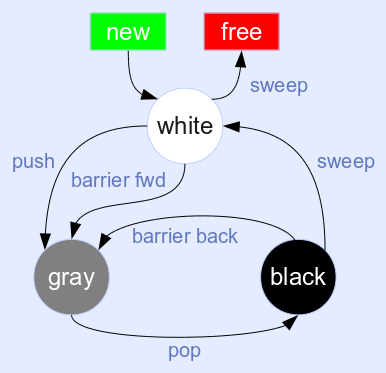
\includegraphics[width=0.4\linewidth]{./gc_color3}
\label{fig:gc_color3}
\end{figure}


Esta es una procedicimiento, en el cual para iniciar la ejecución del recolector de basura, se pausa todos los hilos excepto aquellos que son de utilidad o necesite el recolector. En este este lapso de tiempo, el programa no podrá procesar nada, pero para contrarrestar esta desventaja, STW funciona por un lapso de 10 milisegundos, luego el programa sigue funcionando. Esto es una característica importante, el programa no tiene que esperar hasta que el recolector de basura termine, esto es importante para sistemas de tiempo de ejecución real. Básicamente con esta característica, el recolector procede de a pequeños lapsos de tiempo hasta que termine. Pero para eso, debe ser acompañado de un algoritmo compatible, que así lo es el marcado-y-barrido.

\newpage
\begin{thebibliography}{99}
\bibitem{dec} Nota en The Go Blog sobre la \href{http://blog.golang.org/gos-declaration-syntax}{sintáxis de la declaración}.
\bibitem{pa} FAQ sobre \href{https://golang.org/doc/faq#no_pointer_arithmetic}{aritmética de punteros}.
\bibitem{defer} Effective Go sobre \href{https://golang.org/doc/effective_go.html#defer}{el uso del defer}.
\bibitem{slices} Go blog sobre el \href{http://blog.golang.org/go-slices-usage-and-internals}{uso y los manejos internos de las slices}.
\bibitem{unicode} Artículo de wikipedia sobre \href{https://es.wikipedia.org/wiki/UTF-8}{UTF-8}.
\bibitem{ole} \href{http://dl.acm.org/citation.cfm?id=1243380}{Página de la ACM Library sobre el libro.}
\bibitem{sets} Nota en Go Blog sobre el  \href{http://blog.golang.org/go-maps-in-action}{uso de mapas en Go}.
\bibitem{method_int} FAQ de Go sobre \href{http://golang.org/doc/faq#methods_on_values_or_pointers}{punteros contra valores en los métodos}.
\bibitem{methods_ef} Effective Go sobre \href{https://golang.org/doc/effective_go.html#methods}{métodos}.
\bibitem{implements} FAQ de Go sobre \href{https://golang.org/doc/faq#implements_interface}{por qué no hay ``implements'' en Go}.
\bibitem{video} Video de charla de Google Developers, por Rob Pike, sobre \href{https://www.youtube.com/watch?v=f6kdp27TYZs}{patrones de diseño para concurrencia en Go}.
\bibitem{parvscon} Slides de la charla de Rob Pike \href{http://talks.golang.org/2012/waza.slide#45}{Paralelismo vs Concurrencia} en Go.
\end{thebibliography}

\end{document}